\section{CAD Overview}
\label{sec:CADbackg}
\todointern[inline]{Explain voxelization}
%interaction with it, programs, geometry represenations, datastructures, formats etc., maybe even history if we're overkill
\Acf{CAD} refers to the process of designing a product using a computer system. Until a few decades back, products were designed using a sketch board. It was a challenge to incorporate changes in the construction drafts as well as to keep documentations up to date; hence, it was no surprise that \ac{CAD} systems spread rapidly across all design development branches. They now have irreplaceable use in architecture, mechanical, electrical and civil engineering.

Depending on the discipline, different requirements are set on the virtual model. One may imagine that in a civil engineering model of a building a 2D floor plan is often sufficient; however, in the design of a mechanical motor a 3D model is always necessary. Given these circumstances, various \ac{CAD} software bundles evolved in the different disciplines with completely different modelling approaches. Depending on the discipline, besides the geometry representation, additional parameters such as material properties or manufacturing information are stored. standardized exchange interfaces are employed in order to switch efficiently between different data structures. 

This section presents the relevant geometrical and computational aspects of \ac{CAD} for the project; for a more thorough introduction we refer the reader to \cite{sarcarCAD}.

\subsection{Geometry Representations}
\tododone[inline]{Saumitra: Repetitive use of names, review}
In general, two different ways of describing a geometry are used: a \acf{CSG} or a \acf{BREP}. Other approaches, such as a complete voxelized geometry are not common due to extensive memory consumption.
\subsubsection{Constructive Solid Geometry}
\begin{figure}
\centering
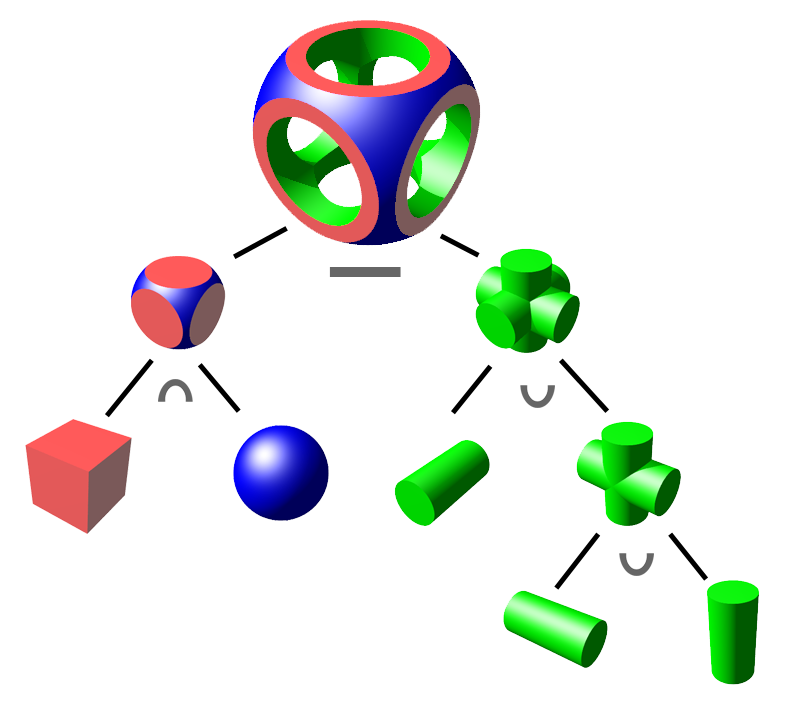
\includegraphics[width=0.5\textwidth]{Pictures/Csg_tree.png}
\caption{\ac{CSG} object tree. The picture shows the construction of a complex object from a cube, a sphere, and a set of cylinders. Figure from \cite{WikipediaCSG}.}
\label{fig:csg_tree}
\end{figure}
The core idea in this format is to start from a set of primitives, e.g. spheres, cylinders and/or cubes. Basic Boolean operations link these primitives towards a complex geometry, as illustrated in \autoref{fig:csg_tree}.

The key advantage of this format is the precise representation using very little storage memory. However, not all desired forms can be represented this format and hence, a second type of geometry description is needed. 
\subsubsection{Boundary Representation}
In this format, instead of storing the geometry information as geometrical objects, only the boundary surfaces of the body are saved. The interior is assumed to be uniformly filled. Especially in complex geometries, this approach simplifies the model to an extent where the amount of data becomes much easier to handle. Surfaces can then be for example stored as a set of triangles (as in \ac{STL} files, see \autoref{subsub:STL} below) or in \ac{NURBS} \acsp{patch} (see \autoref{sec:NURBS}).
Furthermore, holes in the body are made possible by saving the surface normal of the respective boundary. 

By the boundary representation arbitrary geometries can be created. While the data sizes are commonly larger than in \ac{CSG} representation, \ac{BREP} files are usually easier to work with. One also has to keep in mind, that non-physical geometries can result from \ac{BREP} formats through a non-closed surface.

\subsubsection{Voxel Raster}
A very straightforward approach is to store a geometry shape as a regular grid of cubes, so called voxels. In the core, a raster of cubes is placed on the shape, and for each of the voxels the material information is saved. One can imagine that there are various alternatives: a boolean voxel grid, a grid with respective mass densities or saving arbitrary additional information to each voxel. As mentioned before, this representation is not common in CAD systems due to massive memory needs. However, modifications of the representation are more common which mostly deal with saving the shape surface in voxels as treated in \cite{CohenOr1995} or OctTree representations.  

\subsection{Data Exchange Interfaces}
\ac{CAD} software programs usually use their own data formats; in order to exchange models standardized interface formats have been developed. Geometric models are compressed to certain geometry descriptions; transferring additional information, such as material properties or manufacturing information, is in general a difficult task and in some exchange file formats even prohibited. A few common exchange file types are described below, as also compared in \cite{STL}.
\subsubsection{\acs{STL} File Format} \label{subsub:STL}
The \acf{STL} file format describes the model only by its boundary and is thus a \ac{BREP} format. The idea behind its files is simple. The geometric model is discretized into a cloud of points, where sets of three vertices form a triangle; hence, a connected surface of triangles emerges which describes the geometry. The procedure is shown in \autoref{fig:STL} for a two dimensional circle.  
\begin{figure}
\centering
   \scalebox{0.4}{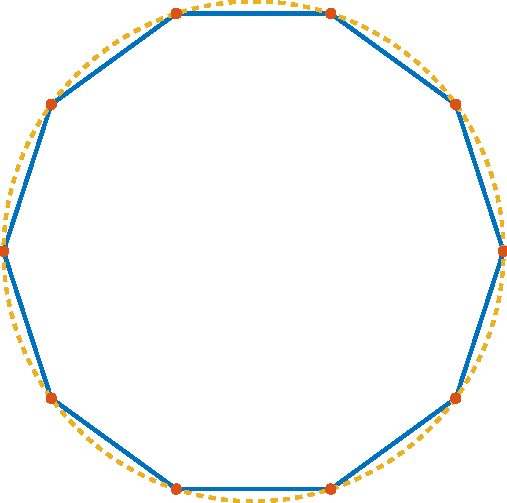
\includegraphics{Pictures/STL.pdf}}\\
   \caption{\ac{STL} discretization for a circle, self-made in MATLAB \cite{MATLAB}. Note that the circle cannot be exactly represented by the vertices and edges.}
   \label{fig:STL}
\end{figure}
The aforementioned triangles boil down to lines in two dimensions. The advantages and disadvantages of this approach become clear: It can be applied to an arbitrary geometry, but accuracy causes difficulties. In order to transfer high precision geometries many vertices are necessary, resulting in big files. Still, as is illustrated in the figure, a perfect circle can never be represented. 

ASCII \ac{STL} files begin with a name and the data on the triangles is constructed as follows: 
\begin{itemize}
\item a facet normal pointing outward
\item a sequence of vertex coordinates
\end{itemize}
As this is the only information provided, no additional data such as material properties are transferred through \ac{STL} files, reducing file size but also range of usage.
\subsubsection{\acs{STEP} and \acs{IGES} File Formats}
To overcome issues of insufficient precision also more elaborate exchange formats exist; these save e.g. a circle as a parameter where no discretization step is involved. Also, the possibility of passing additional parameter information (e.g. density, manufacturing information) is required by certain users. Popular file types that offer these two functionalities are \acf{STEP} and \acf{IGES} files. 

The \ac{STEP} file format is a newly developed data exchange standard and documented in the ISO 10303 norm. On the contrary to \ac{STL} files it uses a combination of \ac{CSG} and \ac{BREP} to store the geometry. Additional information (e.g. density, color) are passed through attribute sets that are stored besides geometry instances (e.g. a circle). A key disadvantage, however, is that they carry much more redundant information \cite{STL}.


The \acl{IGES} is an American National Standard since 1981 to exchange graphics information. Similar to the \ac{STEP} format it uses a combination of \ac{CSG} and \ac{BREP} for the geometry representation. Instead of storing a set of manufacturing information as done in the former, it is built only to exchange graphics information. For example, the \ac{STEP} file transfers a physical density information; in the \ac{IGES} format the only additional parameter stored on a node is the coloring information. Consequentially, file sizes are significantly smaller compared to the \ac{STEP} file format \cite{STL}.

The \ac{IGES} file format contains five different sections: a \emph{Start}, \emph{Global}, \emph{Directory Entry}, \emph{Parameter Data} and \emph{Terminate} section. The \emph{Start} and \emph{Global} section are used for naming and part information. In the \emph{Directory Entry} section additional information like the node color is saved. The \emph{Parameter Data} section is used for storing the coordinate points; the \emph{Terminate} section signals the end of the file \cite{sarcarCAD}.
